\documentclass[11pt]{article}
\usepackage[a4paper,margin=1in]{geometry}
\usepackage{amsmath,amssymb,amsthm,mathtools}
\usepackage{booktabs}
\usepackage{array}
\usepackage{enumitem}
\usepackage{float}
\usepackage{graphicx}
\usepackage{hyperref}
\usepackage[nameinlink,capitalise]{cleveref}
\usepackage[numbers,sort&compress]{natbib}

\newtheorem{theorem}{Theorem}[section]
\newtheorem{proposition}[theorem]{Proposition}
\newtheorem{corollary}[theorem]{Corollary}
\newtheorem{remark}[theorem]{Remark}
\theoremstyle{definition}
\newtheorem{definition}[theorem]{Definition}
\newcommand{\norm}[1]{\left\lVert#1\right\rVert}
\newcommand{\one}{\mathbf 1}
\newcolumntype{L}[1]{>{\raggedright\arraybackslash}p{#1}}

\title{Validated Peripheral Rank-Two Deflation for Repaired Folded-Gaussian Matrices\\
\large Stationary Neumann Solves, Bordered Parity Newton Balls, and Certified Riesz Projectors}
\author{Liang Wang}
\date{July 2026}

\begin{document}
\maketitle

\begin{abstract}
RH-72 replaced the rounded folded-Gaussian rows by exact nonnegative dyadic
stochastic rows and certified their assembly error.  The Perron right vector
is therefore exactly $\one$, but the stationary left vector and the negative
parity Riesz factor remained unvalidated.  This paper closes that finite-scale
spectral gate.

For an exact row-stochastic matrix $A\in\mathbb Q^{n\times n}$, define
\[
 L=I-A^T+\frac1n\one\one^T.
\]
If an approximate inverse $B$ obeys $\norm{I-BL}_F<1$, then $L$ is
invertible.  A single preconditioned residual encloses the normalized
stationary vector and proves that the Perron eigenvalue is simple.  The
negative parity pair is treated as a zero of
\[
 F(r,\lambda)=\binom{Ar-\lambda r}{c^Tr-1}.
\]
For a bordered approximate inverse, the computable inequalities
\[
 \beta+\gamma\rho+M\rho^2\le\rho,
 \qquad \gamma+M\rho<1
\]
give a unique joint eigenpair in the radius-$\rho$ ball.  A second bordered
linear solve validates the left eigenvector at the resulting eigenvalue.
We derive an explicit normalized rank-one projector perturbation bound and
combine it with the stationary factor to enclose the complete rank-two
deflation and the deflated bulk operator.  A Euclidean Grushin/Rouche ledger
independently proves that a radius-$0.01$ circle contains exactly one parity
eigenvalue.

A 160-bit Arb audit covers both fine and Haar-coarse repaired matrices at
$\sigma=0.16,0.08,0.04,0.02,0.01$.  All ten channels close.  The largest
stationary, right-pair, and left-vector errors are respectively
$2.10\times10^{-16}$, $3.54\times10^{-15}$, and
$8.22\times10^{-14}$.  The largest rank-two projector and deflated-bulk
errors are $9.20\times10^{-14}$ and $9.41\times10^{-14}$; the largest
contour transport product is $0.241$.  Gram products, residuals, and final
projector bounds are evaluated from exact dyadic data with outward rounding.

Thus the repaired finite matrices now have certified Perron/parity
rank-two deflations.  The normalized source/observation transfer to RH-70's
frozen Hardy input remains the next gate.  No small-noise uniform theorem,
Stage A1 closure, Hilbert--Polya operator, or Riemann Hypothesis claim is made.
\end{abstract}

\noindent\textbf{Keywords:} stochastic matrix; stationary distribution;
validated eigenpair; Riesz projector; interval arithmetic; Grushin problem.

\medskip
\noindent\textbf{MSC 2020:} 47A10; 47A55; 60J20; 65G20; 65F15.

\section{Introduction}

The RH sequence studies spectral structures generated by a noisy quadratic
map at its first band-merging parameter.  Earlier calculations isolated a
near-$-1$ parity branch and a complementary bulk, but a production-level
certificate must distinguish a floating eigendecomposition from a theorem
about the exact matrix being used.

RH-70 validated a terminal block-Hardy calculation after accepting frozen
binary64 operator, source, and observation arrays as exact dyadic inputs
\citep{WangFrozen2026}.  RH-71 identified the upstream construction of those
arrays as the remaining finite-scale frontier.  RH-72 then certified the
folded-Gaussian kernel, support truncation, normalization, exact stochastic
repair, and Haar assembly \citep{WangAssembly2026}.  In particular, the
repaired matrix satisfies $A\one=\one$ exactly.

The remaining spectral problem is nonnormal.  A small residual alone does not
prove that an eigenpair exists nearby, nor that the corresponding Riesz
projector is well conditioned \citep{Kato1995,Higham2002}.  We therefore use
three separate certificates:

\begin{enumerate}[leftmargin=2.2em]
 \item a linear Neumann certificate for the stationary left vector;
 \item a nonlinear bordered contraction for the right parity eigenpair,
       followed by a linear interval solve for its left partner;
 \item a Grushin/Rouche count on a fixed circle, which records spectral
       isolation independently of a diagnostic eigengap.
\end{enumerate}

The calculations use binary64 only to propose centers.  Every matrix entry and
center coordinate is then converted to its exact dyadic rational, and all
residuals, products, norms, and inequalities are recomputed in Arb
\citep{Johansson2017,Rump2010}.

\subsection*{Contributions}

\begin{enumerate}[leftmargin=2.2em]
 \item We prove and execute a stationary Neumann certificate that also proves
       simplicity of the Perron eigenvalue.
 \item We give a bordered Newton validation for a normalized right eigenpair.
 \item We transfer the validated eigenvalue ball through a bordered left solve.
 \item We derive a projector perturbation formula adapted to the two different
       normalizations used by the right and left systems.
 \item We enclose the rank-two projector and deflated bulk errors.
 \item We close a radius-$0.01$ parity contour count in every fine/coarse
       channel at the five archived noise scales.
\end{enumerate}

\section{Exact repaired matrices and notation}

At each noise scale, RH-72 supplies an exact nonnegative dyadic matrix
$A\in\mathbb Q^{n\times n}$ with
\begin{equation}
 A\one=\one.
 \label{eq:stochastic}
\end{equation}
The fine dimensions are $32,64,128,256,512$.  The coarse matrix is formed by
the exact rational Haar averaging rule
\begin{equation}
 A^{(c)}_{ij}=\frac12\sum_{a,b\in\{0,1\}}A_{2i+a,2j+b}.
 \label{eq:coarse}
\end{equation}
It is again nonnegative and exactly row-stochastic.

All vector norms are Euclidean and all matrix norms in the proofs are
subordinate two-norms.  The implementation may replace a two-norm by the
Frobenius norm, since $\norm X_2\le\norm X_F$.  An overline such as
$\overline x$ denotes a rigorously rounded upper bound, not complex
conjugation.  Transposes may be replaced by adjoints without changing the
arguments.

\section{Stationary Neumann certificate}
\label{sec:stationary}

Put $e=\one$ and
\begin{equation}
 L=I-A^T+\frac1n ee^T,
 \qquad b=\frac1n e.
 \label{eq:stationary-system}
\end{equation}

\begin{theorem}[Stationary Neumann certificate]
\label{thm:stationary}
Let $B$ be any square matrix and suppose
\[
 \gamma=\norm{I-BL}<1.
\]
Then $L$ is invertible.  The vector $\pi=L^{-1}b$ is the unique normalized
stationary vector:
\[
 A^T\pi=\pi,
 \qquad e^T\pi=1.
\]
For any center $\pi_0$, set
\[
 \beta=\norm{B(b-L\pi_0)}.
\]
Then
\begin{equation}
 \norm{\pi-\pi_0}\le\frac{\beta}{1-\gamma}.
 \label{eq:stationary-error}
\end{equation}
Moreover, the eigenvalue $1$ of $A$ is algebraically simple.
\end{theorem}

\begin{proof}
The inequality implies that $BL=I-(I-BL)$ is invertible by the Neumann
series.  Since $B$ and $L$ are square, both are invertible.  Multiplying
$L\pi=b$ on the left by $e^T$ and using $Ae=e$ gives $e^T\pi=1$; substitution
then gives $(I-A^T)\pi=0$.

If $(I-A^T)x=0$ and $e^Tx=0$, then $Lx=0$, hence $x=0$.  Thus the stationary
eigenspace is one dimensional.  Finally, a nonnegative stochastic matrix is
power bounded in the induced infinity norm: $\norm{A^k}_\infty=1$.  A
nontrivial Jordan block at the unit-modulus eigenvalue $1$ would make
$\norm{A^k}$ grow polynomially, so $1$ is semisimple and therefore
algebraically simple.  For the error, write
\[
 \pi-\pi_0=(BL)^{-1}B(b-L\pi_0)
\]
and use $\norm{(BL)^{-1}}\le(1-\gamma)^{-1}$.
\end{proof}

Because the exact Perron right vector is $e$, the approximate Perron
projector $e\pi_0^T$ satisfies
\begin{equation}
 \norm{e\pi^T-e\pi_0^T}
 \le\sqrt n\,\frac{\beta}{1-\gamma}.
 \label{eq:perron-projector}
\end{equation}

\section{Bordered Newton validation of the parity pair}
\label{sec:right}

Let $(r_0,\lambda_0)$ be a numerical negative real eigenpair center and let
$c$ be a fixed numerical left vector scaled so that $c^Tr_0$ is close to one.
Define
\begin{equation}
 F(r,\lambda)=
 \begin{pmatrix}Ar-\lambda r\\c^Tr-1\end{pmatrix},
 \qquad
 J_0=
 \begin{pmatrix}A-\lambda_0I&-r_0\\c^T&0\end{pmatrix}.
 \label{eq:newton}
\end{equation}

\begin{theorem}[Bordered Newton validation]
\label{thm:newton}
Let $B$ be an approximate inverse of $J_0$, and define
\[
 \beta=\norm{BF(r_0,\lambda_0)},\qquad
 \gamma=\norm{I-BJ_0},\qquad M=\norm B.
\]
If a radius $\rho>0$ satisfies
\begin{equation}
 \beta+\gamma\rho+M\rho^2\le\rho,
 \qquad \gamma+M\rho<1,
 \label{eq:newton-gates}
\end{equation}
then $F$ has a unique zero $(r,\lambda)$ in the joint Euclidean ball
$\norm{(r-r_0,\lambda-\lambda_0)}\le\rho$.
\end{theorem}

\begin{proof}
For $h=(u,\eta)$, the nonlinear remainder of $F$ at the center is
$(-\eta u,0)$, whose norm is at most $\norm h^2$.  The preconditioned fixed
point map $h\mapsto h-BF((r_0,\lambda_0)+h)$ therefore maps the radius-$\rho$
ball into itself by the first inequality in \eqref{eq:newton-gates}.  Its
Lipschitz constant there is at most $\gamma+M\rho<1$.  Banach's fixed point
theorem proves existence and uniqueness.
\end{proof}

The implementation takes Frobenius upper bounds for $M$ and $\gamma$.  It
first proposes $2\beta/(1-\gamma)$ and then checks both inequalities in Arb;
no floating decision is accepted without this final interval check.

\section{Left parity validation}
\label{sec:left}

The right Newton normalization gives $c^Tr=1$.  To construct the left mode,
fix the right center $r_0$ and solve, at the unknown validated eigenvalue,
\begin{equation}
 H(\lambda)
 \binom{\ell}{\alpha}
 =\binom0{1},
 \qquad
 H(\lambda)=
 \begin{pmatrix}A^T-\lambda I&c\\r_0^T&0\end{pmatrix}.
 \label{eq:left-system}
\end{equation}

\begin{theorem}[Left parity validation]
\label{thm:left}
Let $B_\ell$ approximately invert $H(\lambda_0)$ and put
\[
 \gamma_\ell=\norm{I-B_\ell H(\lambda_0)},
 \qquad M_\ell=\norm{B_\ell}.
\]
For a center $x_0=(\ell_0,0)$, let
\[
 \beta_0=\norm{B_\ell\{(0,1)^T-H(\lambda_0)x_0\}}.
\]
If $|\lambda-\lambda_0|\le\rho$ and
\begin{equation}
 \Gamma=\gamma_\ell+M_\ell\rho<1,
 \label{eq:left-gate}
\end{equation}
then \eqref{eq:left-system} has a unique solution and
\begin{equation}
 \norm{x-x_0}
 \le
 \frac{\beta_0+M_\ell\rho\norm{\ell_0}}{1-\Gamma}.
 \label{eq:left-error}
\end{equation}
For the eigenvalue supplied by \cref{thm:newton}, its scalar component is
$\alpha=0$; hence $A^T\ell=\lambda\ell$ and $r_0^T\ell=1$.
\end{theorem}

\begin{proof}
The perturbation $H(\lambda)-H(\lambda_0)$ has norm at most $\rho$.
Preconditioning and a Neumann series give \eqref{eq:left-error}.  At the
validated right eigenpair, multiply the first block equation by $r^T$:
\[
 r^T(A^T-\lambda I)\ell+(c^Tr)\alpha=0.
\]
The first term vanishes and $c^Tr=1$, so $\alpha=0$.
\end{proof}

\section{Normalized projector and bulk bounds}
\label{sec:projector}

Write $r=r_0+\delta r$, $\ell=\ell_0+\delta\ell$ and suppose
\[
 \norm{\delta r}\le\varepsilon_r,qquad
 \norm{\delta\ell}\le\varepsilon_\ell.
\]
The left normalization gives $\ell^Tr_0=1$.  Consequently
\[
 |\ell^Tr-1|
 =|\ell^T\delta r|
 \le(\norm{\ell_0}+\varepsilon_\ell)\varepsilon_r
 =:\eta.
\]

\begin{proposition}[Normalized parity projector]
\label{prop:projector}
If $\eta<1$, then the exact parity Riesz projector
$P_-=r\ell^T/(\ell^Tr)$ and the center tensor $Q_0=r_0\ell_0^T$ obey
\begin{equation}
 \norm{P_--Q_0}
 \le
 \frac{N}{1-\eta}
 +\frac{\norm{r_0}\norm{\ell_0}\eta}{1-\eta},
 \label{eq:projector-error}
\end{equation}
where
\[
 N=\varepsilon_r(\norm{\ell_0}+\varepsilon_\ell)
   +\norm{r_0}\varepsilon_\ell.
\]
\end{proposition}

\begin{proof}
The numerator difference satisfies
\[
 \norm{r\ell^T-r_0\ell_0^T}
 \le\varepsilon_r(\norm{\ell_0}+\varepsilon_\ell)
      +\norm{r_0}\varepsilon_\ell=N.
\]
Also $|\ell^Tr|\ge1-\eta$ and
$|1/(\ell^Tr)-1|\le\eta/(1-\eta)$.  Insert and subtract
$r_0\ell_0^T/(\ell^Tr)$.
\end{proof}

Let $P_+=e\pi^T$, $Q_+=e\pi_0^T$, and let $E_+$ and $E_-$ denote the
right sides of \eqref{eq:perron-projector} and
\eqref{eq:projector-error}.  Then
\begin{equation}
 \norm{(P_++P_-)-(Q_++Q_0)}\le E_++E_-.
 \label{eq:rank-two}
\end{equation}
For the exact and center-deflated bulks
\[
 K=A-P_+-\lambda P_- ,
 \qquad K_0=A-Q_+-\lambda_0Q_0,
\]
we also obtain
\begin{equation}
 \norm{K-K_0}
 \le E_++(|\lambda_0|+\rho)E_-
      +\rho\norm{r_0}\norm{\ell_0}.
 \label{eq:bulk}
\end{equation}

\section{Parity contour count}
\label{sec:contour}

The Newton theorem gives a local zero of the normalized eigenproblem.  We
also certify spectral isolation on a fixed, much larger circle.  Let
$z=\lambda_0+w$, $|w|=R$, and use the bordered operator at the center as a
Grushin problem.  Denote by $E_0$ a certified upper bound for its reduced
inverse and by $g_-=\underline{|\ell_0^Tr_0|}$,
$g_+=\overline{|\ell_0^Tr_0|}$.  The RH-42 Euclidean ledger transfers the
bordered inverse to the circle whenever
\begin{equation}
 R E_0<1.
 \label{eq:transport}
\end{equation}
It then bounds the right and left channels, the affine scalar boundary, and
the residual correction.  If the scalar correction is smaller than the
affine boundary, Rouche's theorem gives exactly one zero inside the circle
\citep{WangContour2026}.

In the present audit $R=0.01$.  The Gram interval is not assumed to equal
one: it is recomputed as the exact dyadic dot product of the displayed
centers.  Likewise both residuals are formed against the exact rational
matrix, rather than a rounded dense copy.  This is the parity contour count
used in the archived gate.

\section{Five-scale interval audit}
\label{sec:audit}

SciPy eigensolvers propose $\pi_0,r_0,\ell_0,\lambda_0$ and approximate
inverse centers.  Every binary64 number is converted by its exact integer
ratio.  The repaired fine and coarse matrices are exact fractions.  Arb at
160-bit precision then evaluates all matrix residuals, Frobenius norms,
Neumann denominators, Newton inequalities, Gram products, projector formulas,
and final bulk bounds with outward rounding.

\begin{table}[H]
\centering
\small
\caption{Fine/coarse parity centers and certified rank-two errors.}
\label{tab:main}
\begin{tabular}{@{}rrrrrr@{}}
\toprule
$\sigma$ & $n$ & $\lambda_-^{(f)}$ & $\lambda_-^{(c)}$ &
$E_2^{(f)}$ & $E_2^{(c)}$\\
\midrule
0.16 & 32  & -0.86795414 & -0.86540565 & $3.38\,10^{-14}$ & $1.90\,10^{-14}$\\
0.08 & 64  & -0.93787089 & -0.93675101 & $4.61\,10^{-14}$ & $3.72\,10^{-14}$\\
0.04 & 128 & -0.96563294 & -0.96505988 & $5.00\,10^{-14}$ & $2.75\,10^{-14}$\\
0.02 & 256 & -0.97925977 & -0.97892302 & $5.62\,10^{-14}$ & $4.60\,10^{-14}$\\
0.01 & 512 & -0.98665865 & -0.98645070 & $9.20\,10^{-14}$ & $5.89\,10^{-14}$\\
\bottomrule
\end{tabular}
\end{table}

Here $E_2$ is the complete rank-two projector error from
\eqref{eq:rank-two}.  The corresponding maximum deflated-bulk error is
$9.41\times10^{-14}$.

\begin{table}[H]
\centering
\small
\caption{Fine-channel validation radii and contour transport products.}
\label{tab:radii}
\begin{tabular}{@{}rrrrr@{}}
\toprule
$\sigma$ & stationary error & right radius & left error & $0.01E_0$\\
\midrule
0.16 & $1.50\,10^{-16}$ & $3.30\,10^{-15}$ & $2.54\,10^{-14}$ & 0.0652\\
0.08 & $1.65\,10^{-16}$ & $3.46\,10^{-15}$ & $3.64\,10^{-14}$ & 0.0862\\
0.04 & $1.55\,10^{-16}$ & $2.93\,10^{-15}$ & $4.13\,10^{-14}$ & 0.1196\\
0.02 & $1.07\,10^{-16}$ & $2.49\,10^{-15}$ & $4.87\,10^{-14}$ & 0.1689\\
0.01 & $1.26\,10^{-16}$ & $2.95\,10^{-15}$ & $8.22\,10^{-14}$ & 0.2402\\
\bottomrule
\end{tabular}
\end{table}

Every coarse channel has smaller contour transport than its fine partner.
Across all ten channels the smallest exact-dyadic Gram lower bound exceeds
$0.9999999999999997$, and every Rouche scalar gate is green.  The diagnostic
distance to the remaining numerical spectrum is archived but is not used as
a proof input.

\begin{figure}[H]
\centering
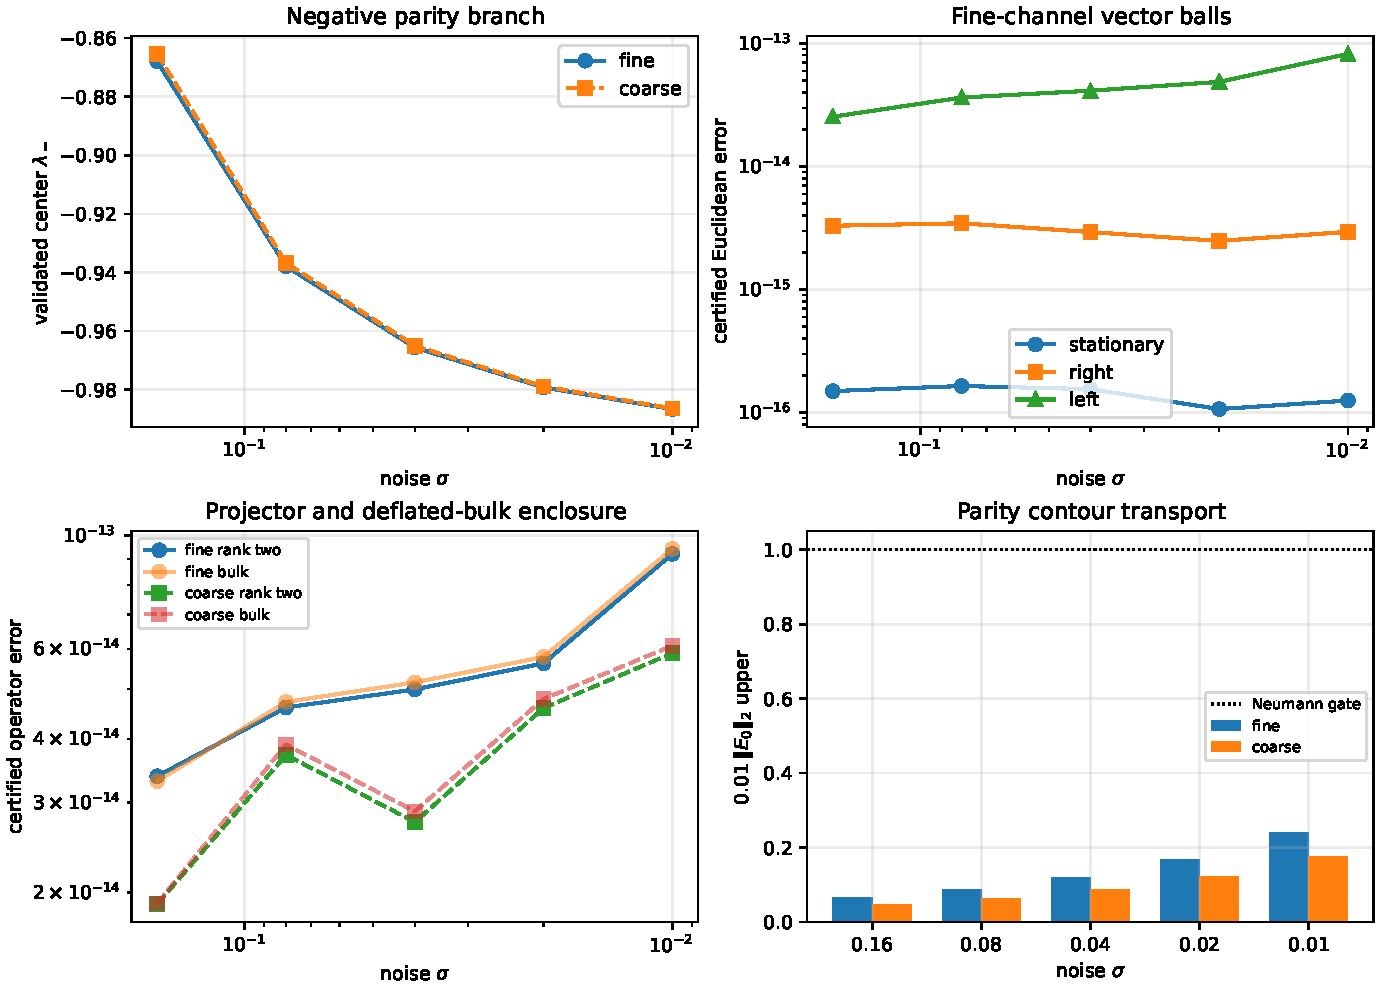
\includegraphics[width=0.98\textwidth]{figures/validated_peripheral_rank_two.pdf}
\caption{Validated parity branch, vector balls, rank-two/bulk enclosures, and
fixed-radius contour transport.  Reversing the horizontal noise axis makes the
small-noise direction run left to right.}
\label{fig:audit}
\end{figure}

\section{What is and is not closed}
\label{sec:boundary}

The result is exact for each archived repaired dyadic matrix.  Together with
RH-72 it removes the following finite-scale gates:

\begin{enumerate}[leftmargin=2.2em]
 \item folded-Gaussian and Haar matrix assembly;
 \item the exact Perron right vector and validated stationary left vector;
 \item the isolated negative parity eigenvalue and both Riesz vectors;
 \item the complete rank-two deflation and its center error.
\end{enumerate}

The next task is the \emph{source/observation transfer}: the parity and
stationary factor balls must be propagated through all normalizations used to
construct the forcing and observation vectors.  The resulting upstream
operator/source/observation triple must then be compared with the frozen triple
accepted by RH-70, and that difference must be inserted into the augmented
Hardy certificate.

This paper is finite-scale.  It does not prove a uniform small-noise
peripheral theorem or a continuum spectral limit.  It does not close Stage A1
or unconditional Stage A4.  It does not construct a self-adjoint
Hilbert--Polya operator, prove a $T\log T$ law or prime-power trace formula,
locate zeta zeros, or prove the Riemann Hypothesis.

\section{Conclusion}

The nonnormal spectral factors of the repaired production matrices can be
certified with compact, independently checkable ledgers.  A stationary
Neumann solve, a bordered Newton ball, a perturbed bordered left solve, and a
fixed-radius Grushin count together turn the numerical Perron/parity split into
a theorem about exact dyadic matrices.  The largest complete rank-two error at
the archived scales remains below $10^{-13}$.

The finite-scale route therefore advances one gate upstream: RH-74 should
validate normalized source and observation construction and execute the full
upstream-to-frozen Hardy bridge.  Whether these constants remain controlled
uniformly as $\sigma\downarrow0$ is deliberately left for later papers.

\bibliographystyle{plainnat}
\bibliography{references}

\end{document}
